% Chapter 1

\chapter{Introducción general} % Main chapter title

En este capítulo se realiza una breve introducción a la necesidad que condujo al desarrollo del trabajo. Se presenta a los sistemas embebidos y el estado del arte de dispositivos similares. Asimismo, se explica el objetivo y los alcances del trabajo.

\label{Chapter1} % For referencing the chapter elsewhere, use \ref{Chapter1} 
\label{IntroGeneral}

%----------------------------------------------------------------------------------------

% Define some commands to keep the formatting separated from the content 
\newcommand{\keyword}[1]{\textbf{#1}}
\newcommand{\tabhead}[1]{\textbf{#1}}
\newcommand{\code}[1]{\texttt{#1}}
\newcommand{\file}[1]{\texttt{\bfseries#1}}
\newcommand{\option}[1]{\texttt{\itshape#1}}
\newcommand{\grados}{$^{\circ}$}

%----------------------------------------------------------------------------------------

%\section{Introducción}

%----------------------------------------------------------------------------------------
\section{Sistemas embebidos en la agricultura}

En las últimas décadas, la cosecha de kiwi ha experimentado un notable proceso de transformación, impulsado por la integración de tecnologías como los sistemas embebidos. Estos sistemas, capaces de realizar tareas específicas en tiempo real, se han vuelto fundamentales en la modernización de este sector.

Por otra parte, una de las actividades clave consiste en estimar, lo más exactamente posible, la producción total, ya que esto condiciona un conjunto importante de aspectos logísticos que deben ser atendidos correctamente durante la recolección.

Actualmente, el volumen de cosecha se estima al contar los frutos por unidad de superficie en una etapa avanzada de desarrollo. Sin embargo, esta evaluación tardía es demasiado cercana a la cosecha y muy dificultosa en plantaciones grandes.

Es en este contexto, que el prototipo KiwiScan permite recolectar imágenes de la plantación con el fin de realizar una detección de objetos. De esta forma, se obtiene una estimación de los frutos para facilitar la toma de decisiones operativas y estratégicas \citep{Mendoza2021}.

\subsection{Requerimientos del sistema}

Se detallan los requerimientos del sistema, con las funcionalidades y características necesarias para cumplir con los objetivos del proyecto.

\begin{enumerate}
	\item Requerimientos funcionales:
		\begin{enumerate}
			\item El sistema debe registrar la temperatura del ambiente.
			\item El sistema debe registrar la humedad del ambiente.
			\item El sistema debe informar el espacio disponible de la tarjeta microSD.
            \item El sistema debe informar la cantidad de fotos tomadas.
		\end{enumerate}
	\item Requerimientos no funcionales:
		\begin{enumerate}
			\item El sistema debe ser escalable, de forma de poder agregar más sensores en el futuro.
			\item El firmware debe estar modularizado.
            \item El firmware debe estar sobre un sistema operativo.
		\end{enumerate}
    \item Requerimientos de interfaz gráfica en la pantalla LCD:
		\begin{enumerate}
			\item Se debe mostrar los valores de humedad y temperatura.
			\item Se debe mostrar el espacio disponible en la tarjeta microSD.
            \item Se debe mostrar la cantidad de fotos tomadas.
            \item La información en pantalla debe actualizarse cada 5 segundos.
		\end{enumerate}
    \item Requerimientos de interoperabilidad:
		\begin{enumerate}
			\item Las fotos deben almacenarse en un formato de archivo JPG o JPEG.
			\item Las imágenes capturadas deben tener un mínimo de resolución de 640 x 480.
            \item Cada imagen guardada no debe superar los 10 MB.
		\end{enumerate}
    \item Requerimientos de documentación:
		\begin{enumerate}
			\item Todo el código fuente debe estar comentado.
			\item Se debe presentar un informe de avance del proyecto.
		\end{enumerate}
\end{enumerate}

%----------------------------------------------------------------------------------------

\section{Estado del arte}

Durante la etapa de investigación del trabajo, se realizó una búsqueda de productos comerciales en el mercado local e internacional. Se encontraron algunos con características similares al que se pretende desarrollar. Un dato interesante a resaltar es que todos los productos hallados provienen del mercado internacional; no se identificó ningún producto o empresa que ofrezca este tipo de soluciones en el mercado local hasta el momento. A continuación, se describen los hallazgos encontrados.

\subsection{Fruitometry}

La tecnología de estimación digital de cultivos (DCE) de Fruitometry que se muestra en la figura \ref{fig:Fruitometry}, permite a los productores y administradores de huertos observar el desempeño de su cultivo durante la temporada de cosecha. Esto ayuda a maximizar los rendimientos, reducir los costos de cultivo y proporcionar estimaciones antes de la recolección.

Las unidades de campo, montadas en cuatriciclos y vehículos todo terreno, contienen una variedad de cámaras y sensores que capturan información sobre la densidad de cultivos y las características del huerto. Para cada escaneo de la plantación, se toman miles de fotografías. Luego, estas se procesan en tiempo real mediante el motor de inteligencia artificial con aprendizaje profundo para identificar brotes, flores, frutos y características de interés.

Este conjunto de datos se utiliza para crear un mapa de calor de densidad resumido y generar informes que se usan para tomar decisiones sobre cómo mejorar el rendimiento del huerto, identificar áreas que requieren atención y dirigir la mano de obra hacia ellas \citep{WEBSITE:Fruitometry2024}.

\vspace{1cm}
\begin{figure}[htbp]
	\centering
	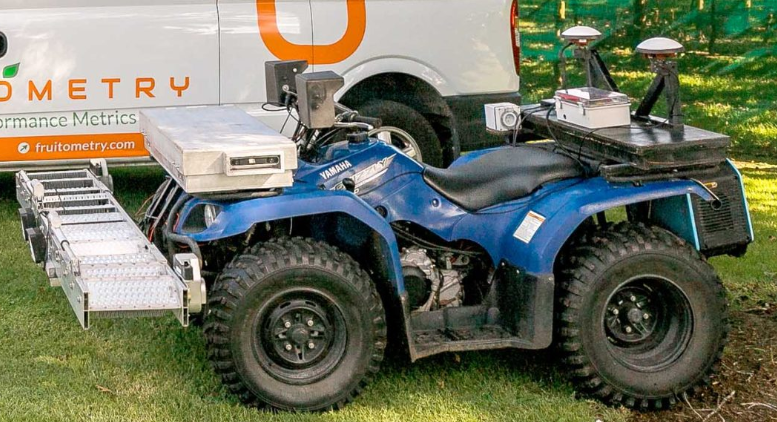
\includegraphics[width=.5\textwidth]{./Figures/Fruitometry.png}
	\caption{Unidad de campo Fruitometry\protect\footnotemark.}
	\label{fig:Fruitometry}
\end{figure}
\vspace{1cm}

\footnotetext{Imagen tomada de \url{https://fruitometry.com/about-fruitometry/}}

\subsection{Detección de kiwis en imágenes de campo}

En un trabajo de investigación realizado en la Universidad Yangling, China, se capturaron imágenes de kiwis en un huerto bajo diferentes condiciones de iluminación y en distintos momentos del día: mañana, tarde y noche, tanto con flash como sin él. Estas fotografías fueron empleadas para la detección de objetos mediante un modelo llamado Faster R-CNN, implementado con la arquitectura VGG16. Después de aplicar las detecciones, el modelo alcanzó una precisión promedio del 87,61 \%. En la figura \ref{fig:Song2019} se muestran los resultados obtenidos.

Este sistema de visión artificial resultó ser eficaz en la detección de diferentes categorías de frutos en el campo y actuó como un soporte fundamental al robot cosechador. Equipado con este sistema, el robot operó de manera continua durante la temporada de cosecha, lo que representó un avance significativo hacia la automatización de la recolección agrícola \citep{Song2019}.

\vspace{1cm}

\begin{figure}[htbp]
	\centering
	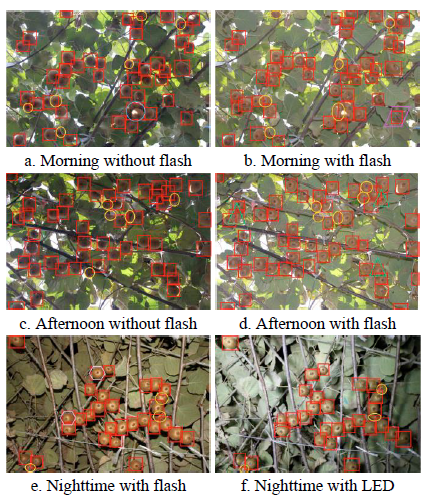
\includegraphics[width=.5\textwidth]{./Figures/Song2019.png}
	\caption{Resultados de una detección de objetos\protect\footnotemark.}
	\label{fig:Song2019}
\end{figure}

\vspace{1cm}
\footnotetext{Imagen tomada de "Kiwifruit detection in field
images using Faster R-CNN with VGG16"}

\newpage
\subsection{Calibrado de frutas}

Existen diversos productos comerciales que aplican la detección de objetos para llevar a cabo procesos de clasificación y calibrado de frutas u hortalizas. Estas máquinas, diseñadas específicamente para grandes cadenas de distribución, automatizan la selección y el empaquetado de los productos, lo que incrementa la eficiencia y reduce los tiempos operativos. El sistema funciona a través de una cinta transportadora equipada con cámaras, que capturan imágenes en tiempo real de cada elemento \citep{WEBSITE:Unitec2024}.

Además de identificar cada objeto, las cámaras registran una serie de parámetros importantes, como el diámetro, la longitud, la forma y, en algunos casos, el color. Estos datos se procesan con algoritmos de visión artificial, que clasifican los productos según criterios preestablecidos de calidad.

%----------------------------------------------------------------------------------------

\section{Objetivo y alcances}


En la siguiente sección se describen los objetivos del proyecto, los alcances y los aspectos no considerados en el desarrollo del prototipo.

\subsection{Objetivo}

El objetivo del presente trabajo es el desarrollo e implementación de un prototipo que permita contabilizar el rendimiento esperado de un lote de producción de kiwi en forma temprana, a través del procesamiento de imágenes.

\subsection{Alcances contemplados}
El alcance establecido para el trabajo incluyó las siguientes tareas:

\begin{itemize}
\item Implementación de un prototipo funcional que toma fotografías de forma automática.
\item Desarrollo del firmware sobre un sistema operativo de tiempo real.
\end{itemize}

\subsection{Aspectos no incluidos en el prototipo}

El alcance establecido para el trabajo no incluye las siguientes tareas:

\begin{itemize}
\item Desarrollo del modelo de detección de objetos.
\item Recolección de imágenes para el proceso de entrenamiento.
\item Pruebas de funcionamiento en la plantación.
\end{itemize}

%----------------------------------------------------------------------------------------
